\documentclass[a4paper]{arrowhead}

\usepackage[utf8]{inputenc}
\usepackage[table]{xcolor}
\usepackage{tcolorbox}
\usepackage[yyyymmdd]{datetime}
\usepackage{multirow}
\renewcommand{\dateseparator}{-}

\usepackage{bera}% optional: just to have a nice mono-spaced font
\usepackage{listings}
\usepackage{xcolor}

\colorlet{punct}{red!60!black}
\definecolor{background}{HTML}{EEEEEE}
\definecolor{delim}{RGB}{20,105,176}
\colorlet{numb}{magenta!60!black}

\lstdefinelanguage{json}{
    basicstyle=\normalfont\ttfamily,
    numbers=left,
    numberstyle=\scriptsize,
    stepnumber=1,
    numbersep=8pt,
    showstringspaces=false,
    breaklines=true,
    frame=lines,
    backgroundcolor=\color{background},
    literate=
     *{0}{{{\color{numb}0}}}{1}
      {1}{{{\color{numb}1}}}{1}
      {2}{{{\color{numb}2}}}{1}
      {3}{{{\color{numb}3}}}{1}
      {4}{{{\color{numb}4}}}{1}
      {5}{{{\color{numb}5}}}{1}
      {6}{{{\color{numb}6}}}{1}
      {7}{{{\color{numb}7}}}{1}
      {8}{{{\color{numb}8}}}{1}
      {9}{{{\color{numb}9}}}{1}
      {:}{{{\color{punct}{:}}}}{1}
      {,}{{{\color{punct}{,}}}}{1}
      {\{}{{{\color{delim}{\{}}}}{1}
      {\}}{{{\color{delim}{\}}}}}{1}
      {[}{{{\color{delim}{[}}}}{1}
      {]}{{{\color{delim}{]}}}}{1},
}



\begin{document}

%% Arrowhead Document Properties
\ArrowheadTitle{The Arrowhead OPC-UA to REST Proof-of-concept --- System Description}
\ArrowheadType{PUBLIC}
\ArrowheadVersion{0.1}
\ArrowheadDate{\today}
\ArrowheadAuthor{Niklas Karvonen}
\ArrowheadStatus{DRAFT}
\ArrowheadContact{niklas.karvonen@ltu.se}
\ArrowheadFooter{\href{www.arrowhead.eu}{www.arrowhead.eu}}
\ArrowheadSetup
%%

%% Front Page
\begin{center}
  \vspace*{1cm}
  \LARGE{\arrowtitle}
  \vspace*{1cm}
  \vspace*{\fill}

  % Front Page Image
  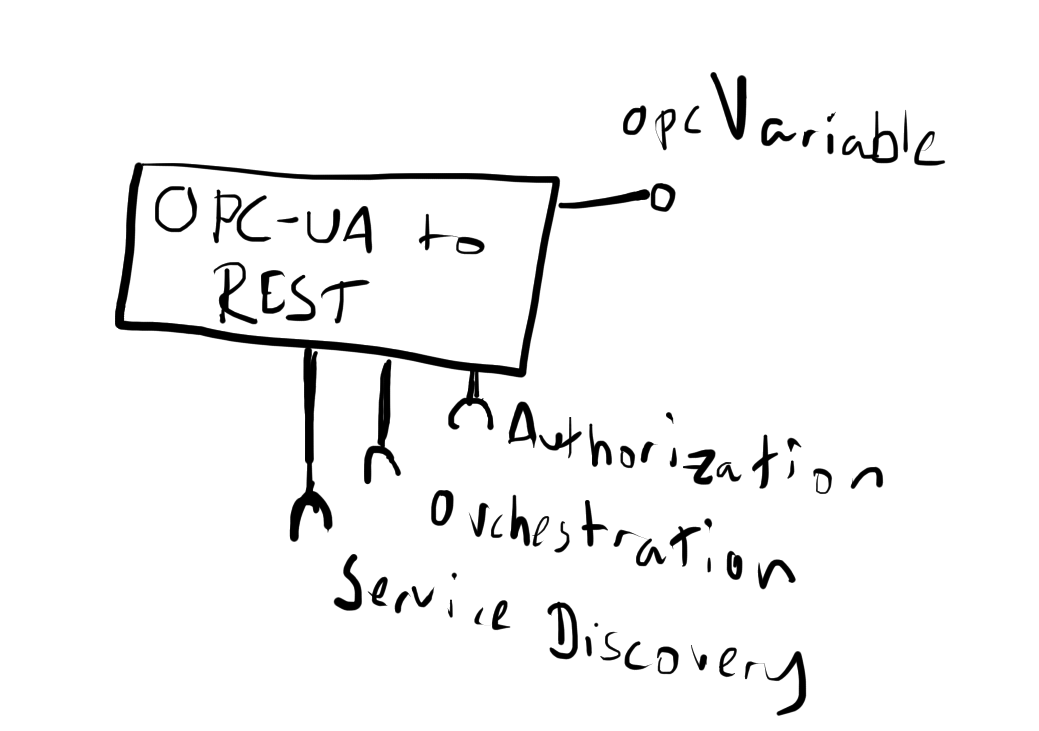
\includegraphics[scale=1.5]{fig/OPC-2-REST_SysD.png}

  \vspace*{1cm}
  \vspace*{\fill}

  % Front Page Abstract
  \begin{abstract}
    This document provides the description of a proof-of-concept OPC-UA Provider for the Arrowhead framework. When a Consumer makes a pull-request to the Provider, the Provider connects to an OPC-UA system and reads the requested variable which it then returns in a JSON format to the Consumer.
  \end{abstract}
\end{center}

\newpage

\section{Basic operation}
To start the Provider, run: "java -jar provider-4.0.jar -auth" after building the Maven module. The -auth flag is optional and will only add the Consumer found in the "tester" folder to the IntraCloud authorization so that it can consume the service. If you don't need that, you can omit the -auth flag.
\newline

When the Provider is run, the first thing that it will do is to register itself with the Service Registry. This is done by sending a "Service Registry Entry" to the Service Registry core service. In more detail, this is achieved by sending a JSON object to URI:\textit{serviceregistry/register}. An example of such a Service Registry Entry is found below:

\begin{lstlisting}[language=json,firstnumber=1]
{
  "providedService" : {
    "serviceDefinition" : "OPCUARead",
    "interfaces" : [ "JSON" ],
    "serviceMetadata" : {
      "unit" : "unit"
    }
  },
  "provider" : {
    "systemName" : "InsecureOPCUA2RESTProvider",
    "address" : "127.0.0.1",
    "port" : 8460
  },
  "serviceUri" : "opcVariable",
  "version" : 1
}
\end{lstlisting}

The second thing that the Provider does is that it adds a Consumer called "client1" that is allowed to consume the service IntraCloud. This is done by sending an "IntraCloud Auth Entry" to the Authentication core service. In more detail, this is achieved by sending a JSON object to URI: \textit{authorization/mgmt/intracloud}. An example of an IntraCloud Auth Entry can be found below:

\begin{lstlisting}[language=json,firstnumber=1]
{
  "consumer" : {
    "systemName" : "client1",
    "address" : "localhost",
    "port" : 8080
  },
  "providerList" : [ {
    "systemName" : "InsecureOPCUA2RESTProvider",
    "address" : "127.0.0.1",
    "port" : 8460
  } ],
  "serviceList" : [ {
    "serviceDefinition" : "OPCUARead",
    "interfaces" : [ "JSON" ],
    "serviceMetadata" : {
      "unit" : "unit"
    }
  } ]
}
\end{lstlisting}

Once these registrations are complete, the Provider will listen for incoming requests from Consumers wanting to read OPC-UA variables. A Consumer can read an OPC-UA variable by making a HTTP GET request to the Provider sending it the OPC-UA endpoint, namespace, and variable it wishes to read. These values are sent as URL parameters in the following way: GET opcVariable/\{address\}/\{namespace\}/\{variableName\}. Here "address" is the IP and port to the OPC-UA endpoint, "namespace" is the OPC-UA namespace one wishes to use, and "variableName" is the name of an variable within that namespace wrapped in double quotation marks (you might need to URL encode these using \%22). An example of such an GET request to read the variable xBG5 in namespace 3 can be found below:

\begin{tcolorbox}[colback=white!5!white,colframe=black!75!black,title=HTTP GET that is sent to the Provider]
\{providerIP:port\}/opcVariable/10.48.134.10:4840/3/\%22xBG5\%22
\end{tcolorbox}

When the Provider has received a request, it will first see if there is already an open connection to that endpoint. If not it will connect to the endpoint and keep that connection until the Provider is shut down. Then, it will read the requested variable and return its value, type and timestamp in a JSON format.


\section{Services}
\label{sec:services}

The system consists of a single Provider (but a test Consumer is included in the "tester" folder). This section briefly explains the single service offered by this Provider.

\begin{figure}[h]
  \center
  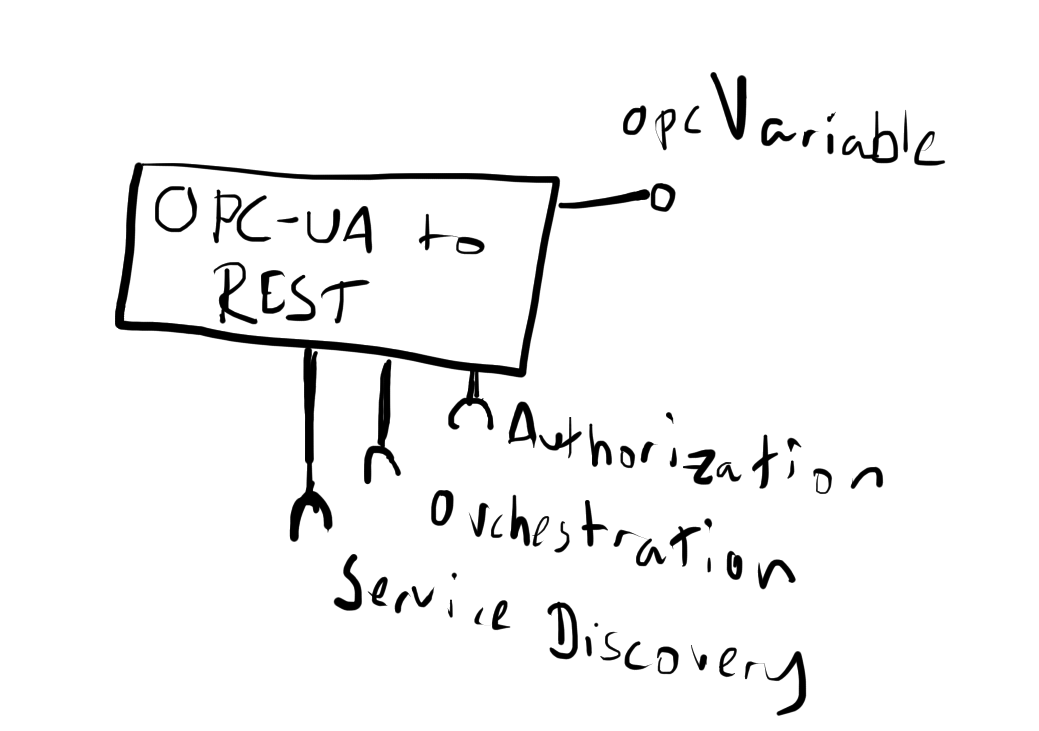
\includegraphics[scale=1.2]{fig/OPC-2-REST_SysD.png}
  \caption{The system consumes the three basic Arrowhead core systems.}
  \label{fig:sysd}
\end{figure}

\subsection{Produced Services}
\noindent\begin{tabularx}{\textwidth}{| p{5.8cm} | X |} \hline
\rowcolor{gray!33} Service & IDD Document Reference \\ \hline

opcVariable                  & Arrowhead IDD OPC-UA-2-REST.pdf \\ \hline

\end{tabularx}


\subsection{Consumed Services}
\noindent\begin{tabularx}{\textwidth}{| p{5.8cm} | X |} \hline
\rowcolor{gray!33} Service & IDD Document Reference \\ \hline

ServiceDiscovery           & {\small\textit{(Not Available)}} \\ \hline
Orchestration              & {\small\textit{(Not Available)}} \\ \hline
AuthorisationControl       & {\small\textit{(Not Available)}} \\ \hline

\end{tabularx}
\vspace*{\baselineskip}

The system consumes the \texttt{ServiceDiscovery}, \texttt{Orchestration} and \texttt{AuthorizationControl} services in order to allow service lookup, determine what services to connect to, and regulate service access, respectively.

\newpage

\section{Use Cases}
\label{sec:use-cases}
\subsection{Monitoring an OPC-UA facility}
This Provider can be used in order for a developer to monitor different variables in an OPC-UA facility. The "tester" Client (found in the tester module) can serve as a starting point for reading OPC-UA variables and can be extended by the developer to include logging, alarms, fault-detection and more.


\section{Behavior Diagrams}
\label{sec:behavior}

\begin{figure}[h]
  \center
  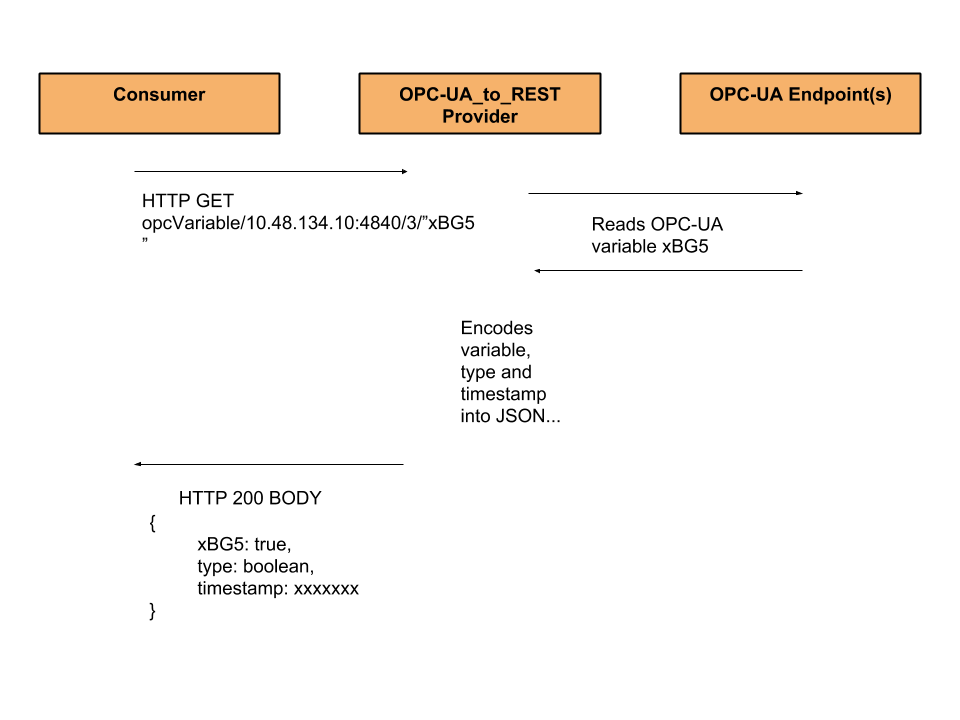
\includegraphics[scale=0.4]{fig/SysD - Sequence diagram.png}
  \caption{Sequence diagram of a Client's interaction with OPC-2-REST Provider}
  \label{fig:sysd}
\end{figure}

\newpage

\section{Security}
\label{sec:security}
The OPC-UA connection does not use any security per default in order to provide a low-complexity example. It is up to the developer to take appropriate actions for securing both the Arrowhead Provider in a secure cloud, and to configure and implement the desired OPC-UA security if this is to be extended into a real implementation.


\newpage

\section{Unsolved Specification Issues}

There are several issues that have not been addressed in this version.
These issues include, but are not limited to, the following:

\begin{itemize}
  \item \textbf{Disconnecting from the OPC-UA} In this version the only way the Provider will disconnect from an OPC-UA endpoint, is when the Provider is shut down. Any connection opened to serve a Client with an OPC-UA variable will remain persistent throughout the lifetime of the Provider.
\end{itemize}

\newpage

\bibliographystyle{IEEEtran}
\bibliography{bibliography}

\newpage

\section{Revision History}
\subsection{Amendments}

\noindent\begin{tabularx}{\textwidth}{| p{1cm} | p{3cm} | p{2cm} | X | p{4cm} |} \hline
\rowcolor{gray!33} No. & Date & Version & Subject of Amendments & Author \\ \hline

1 & & & & \\ \hline

\end{tabularx}

\subsection{Quality Assurance}

\noindent\begin{tabularx}{\textwidth}{| p{1cm} | p{3cm} | p{2cm} | X |} \hline
\rowcolor{gray!33} No. & Date & Version & Approved by \\ \hline

1 & & & \\ \hline

\end{tabularx}

\end{document}